\documentclass[a4paper,english]{ifimaster}
\usepackage[utf8]{inputenc}
\usepackage{babel,duomasterforside}
\usepackage{hyperref}
\usepackage{pdfsync}
\usepackage{minted}
\usepackage{varioref}
\usepackage{amsmath,tabularx}
\usepackage[backend=biber,sortcites]{biblatex}
\usepackage{csquotes}

\newcommand{\todo}[1]{\textcolor{red}{[[TODO: #1]]}\PackageWarning{TODO:}{#1!}}

\newcommand{\timepoint}[1]{t$_#1$}

\addbibresource{citations.bib}

\title{Master Essay}
\author{Ida Sandberg Motzfeldt}
\synctex=1

\begin{document}

\maketitle
\newpage

\frontmatter{}

\tableofcontents

\mainmatter{}

\chapter{Introduction}%
\label{cha:introduction}

Software engineering methodologies for highly-variable software systems lack support for planning the long-term evolution of software. We address this lack in the context of software product lines.

While concepts exist for the construction of software product lines (SPLs), evolution is performed mostly as an informal procedure relying on the intuition and experience of individual engineers with, at most, medium-term goals in mind. The lack of long-term planning for SPL evolution creates a risk of significantly increased development costs, deviation from intended development direction in collaborative efforts and, ultimately, missing long-term goals, which potentially causes a loss of clients and market shares for SPL vendors due to not addressing market needs properly.

When inserting new planned modifications in between the current and a future planned state of the feature model, these changes may cause the original evolution goal to no longer be reachable, e.g., planning to refine a then-deleted feature. Detecting this evolution paradoxes is challenging due to the inherent complexity of the configuration knowledge but is made significantly more complex due to the notion of time present in evolution planning.

To counter these issues, we devise an approach for allowing dynamic changes to an evolution plan while being able to identify evolution paradoxes caused in the future. To achieve this, we will define a formal semantics for how evolution plans can be changed and develop a modular static analysis method to guarantee soundness of the changes.

\chapter{Background}%
\label{cha:background}

\section{Software product lines}%
\label{sec:software-product-lines}

A software product line (SPL) is a family of closely related software systems. These systems can have several features in common, as well as features specific to one or more systems. They are used to make highly configurable systems, where a final product, called a \emph{variant}, is defined by a configuration that consists of a set of selected features. 

There exist several SPL engineering methodologies to implement a whole software product line. These methodologies capitalize on the similarities and differences between the various variants. Instead of developing and maintaining several code bases for each variant, these methodologies combine all these code bases by explicitly encoding their similarities and differences. This makes it easier to develop and maintain features across projects.


\section{Feature Models}
\label{sec:feature-models}

\begin{figure}
  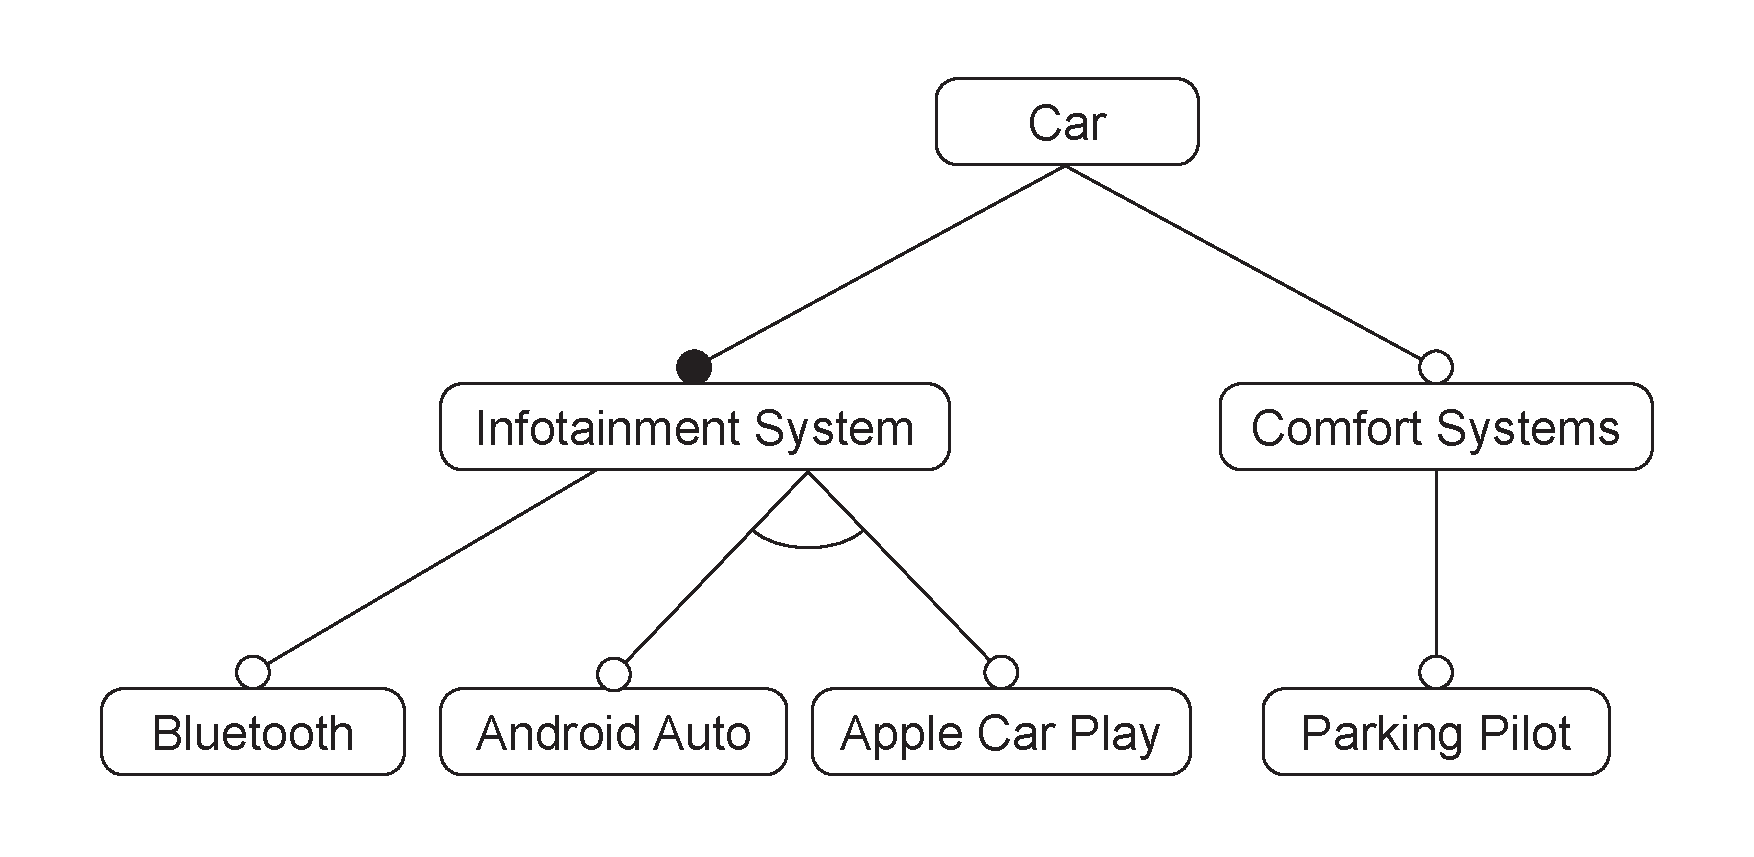
\includegraphics[width=\textwidth]{illustrations/example.pdf}
  \caption{Example feature model \label{fig:feature-model}}
\end{figure}

All the possible variants of a software product line can be defined in terms of a \emph{feature model}. The feature model describes dependencies between features, and how they are related to each other. A feature model is a tree structure, where each vertex represents a feature, and a feature can contain \emph{groups} of more features. See figure \vref{fig:feature-model} for an example of a (simplified) feature model. The small black dot above \texttt{Infotainment System} means that the feature is \emph{mandatory}, which means it must be selected for all variants where its parent feature (here \texttt{Car}) is selected. A white dot (as seen above the \texttt{Bluetooth} feature) means that the feature is \emph{optional}, and does not have to be selected in a variant. The white triangle connecting \texttt{Android Auto} and \texttt{Apple Car Play} is a visualization of an alternative group, or \textit{XOR} group. This means that exactly one of \texttt{Android Auto} and \texttt{Apple Car Play} must be selected. A black triangle (not shown here) is the syntax for the \textit{OR} group, where at least one feature in the group must be selected in a variant. The \textit{AND} group is not shown explicitly, but if it is not an \textit{XOR} or \textit{OR} group, it is an \textit{AND} group. An \textit{AND} group gives no restrictions on which features can be selected.

All features have an associated ID (not shown in example), a name, a (possibly empty) collection of subgroups, and a \emph{feature variation type} (optional or mandatory as explained above). All groups have an associated ID (not shown in example), a \textit{group variation type} (\textit{AND}, \textit{OR}, or \textit{XOR} as explained above), and a collection of subfeatures.

There are some rules for feature models: 
\begin{itemize}
  \item The root feature must be mandatory - it must be selected in all variants
  \item All IDs and names are unique
  \item If a group has group variation type \textit{XOR} or \textit{OR}, it cannot contain any mandatory features.
\end{itemize}
In addition, it is common to define \emph{cross-tree constraints} when there are dependencies that cannot be visualized in a tree; e.g. \texttt{Parking Pilot} cannot be selected without \texttt{Bluetooth} being selected.
\section{Evolution planning}
\label{sec:evolution-planning}
The current tools only deal with the construction of SPLs, and not the evolution. On large software product lines, the planning of long term evolution is lacking, and thus creating a risk of increased development costs. 

\begin{figure}
  \centering
  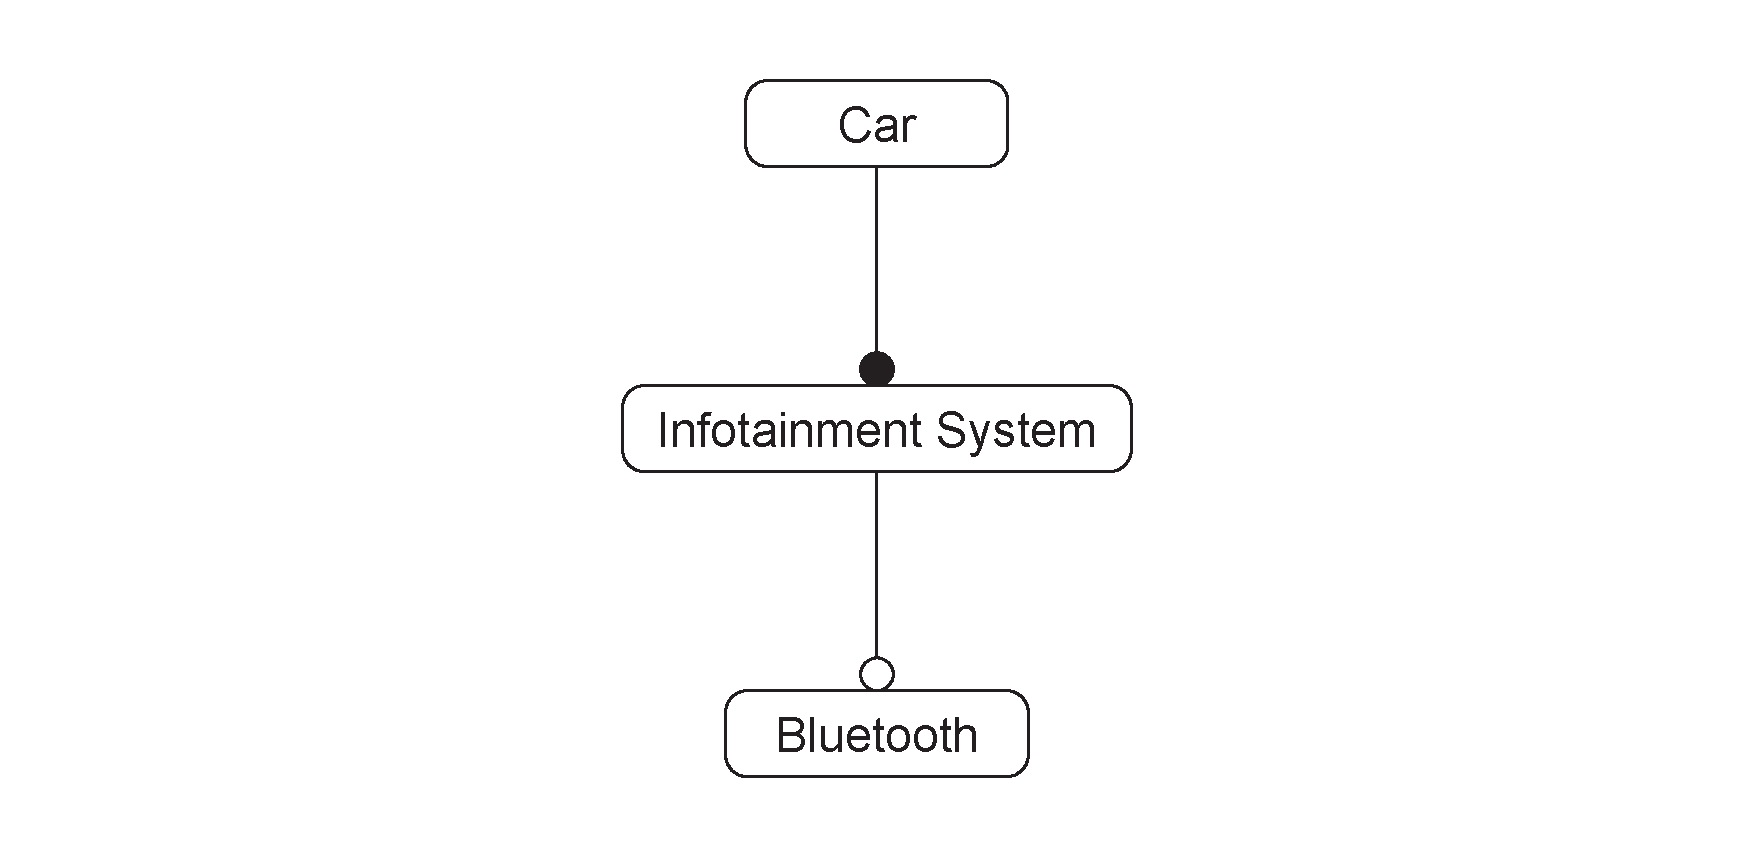
\includegraphics[width=\textwidth]{illustrations/initial.pdf}
  \begin{tabular}{l}
    \textbf{At time 1:}                                           \\ \hline
    add an \textit{XOR} group to \texttt{Infotainment System}.                      \\
    add feature \texttt{Android Auto} to the \texttt{Infotainment System} \textit{XOR} group \\
    add feature \texttt{Car Play} to the \texttt{Infotainment System} \textit{XOR} group     \\
                                                                  \\
    \textbf{At time 2:}                                           \\ \hline
    add an \textit{AND} group to \texttt{Infotainment system} \\
    add feature \texttt{Bluetooth} to the \texttt{Infotainment System} \textit{AND} group \\
    add an \textit{AND} group to \texttt{Comfort Systems}                           \\
    add feature \texttt{Parking Pilot} to the \texttt{Comfort Systems} \textit{AND} group
  \end{tabular}
  \caption{Example evolution plan}
  \label{fig:feature-plan}
\end{figure}
An evolution plan is an initial feature model, followed by an ordered list of plans associated with time points. An example evolution plan is the initial feature model followed by the plan shown in figure \vref{fig:feature-plan}.

Implementing this plan results in the feature model shown in figure \vref{fig:feature-model}.

\subsection{Changing a plan}
\label{sub:changing-a-plan}
As with most large-scale projects, it is often necessary to change the evolution plan for an SPL along the way, due to new requirements or unforeseen circumstances.
Evolution plans for SPLs can grow very large and complex, and consequently it can be challenging to discover paradoxes resulting from plan changes.
It is therefore hugely important that there exist support to do this in the simplest way possible, and the solution must be efficient and scalable due to the size and complexity of software product lines.

\newpage
\subsection{Example evolution paradox}
\label{sub:example-evolution-paradox}
Due to financial difficulties, an example car manufacturer is obliged to cut costs for their planned car SPL (see figure \vref{fig:feature-plan}).
As it results from a short-notice decision, the car system is supposed to drop its stand-alone \texttt{Infotainment} system.
Instead, the car manufacturer decides to focus on a docking station in combination with more sophisticated \texttt{Bluetooth} functionality.
%the introduction of all \texttt{Infotainment} functionality is thus supposed to be postponed.
For the FM evolution plan, this requires replanning activity:
The manufacturer retroactively plans to delete the feature \texttt{Infotainment} at the new intermediate time point \timepoint{0.5}, after the initial version for \timepoint{0} and before the originally planned version for \timepoint{1}.%(arrow \diamonded{3} in \autoref{fig:paradox}).


It is important to note that retroactively inserting intermediate edit operations entails specific challenges due to the different orders of devising and scheduling changes. When devising the changes of the example, their order is as follows:

\begin{enumerate}
	\item [\timepoint{0}:] Plan initial car system.
	\item [\timepoint{1}:] Plan to add \texttt{Bluetooth} feature as child of \texttt{Infotainment}.
	\item [\timepoint{0.5}:] Replan to delete \texttt{Infotainment}.
\end{enumerate}
In contrast, the order in which these changes are scheduled (supposed to be implemented) is the temporal order of all planned changes:
\begin{itemize}
	\item [\timepoint{0}:] Plan initial car system.
	\item [\timepoint{0.5}:] Replan to delete \texttt{Infotainment}.
	\item [\timepoint{1}:] Plan to add \texttt{Bluetooth} feature as child of \texttt{Infotainment}.
\end{itemize}

%%These orders differ whenever FM evolution is replanned with intermediate edit operations.
%Hence, replanning requires two consecutive phases to maintain an overall FM evolution plan:
%First, the new intermediate edit operation is introduced to the evolution plan (arrow \diamonded{3} in \autoref{fig:paradox}).
%Second, all previously devised, yet subsequently scheduled edit operations must be incorporated into the replanned state of the FM evolution plan (arrow \diamonded{4}).

However, incorporating subsequently scheduled edit operations can fail and, thus, damage the structural consistency of an FM evolution plan:
In the car example, the planned change for \timepoint{1} to add \texttt{Bluetooth} as child feature of \texttt{Infotainment} can no longer be implemented as, once reaching \timepoint{1}, the \texttt{Infotainment} feature will have been deleted in the previous \timepoint{0.5}.
The reason for this problem is that the replanned FM evolution plan is structurally inconsistent as an evolution paradox was introduced into the evolution plan of the car SPL with the retroactive intermediate change at \timepoint{0.5}.

\section{Static analysis}
\label{sec:static-analysis}
In \citetitle{book:principles-of-program-analysis} (\citeyear{book:principles-of-program-analysis}), \citeauthor*{book:principles-of-program-analysis} give the following introduction to static analysis:
\begin{displayquote}[\autocite*{book:principles-of-program-analysis}][.]
Program analysis offers static compile-time techniques for predicting safe and computable approximations to the set of values or behaviours arising dynamically at run-time when executing a program on a computer
\end{displayquote}
There are various methods and applications for static analysis, including Data Flow Analysis, Control Flow Analysis, Abstract Interpretation, and Type and Effect Systems \parencite{book:principles-of-program-analysis}. Static analysis provides methodologies for validating software. Due to the inherent undecidability of program behaviour, the methods tend to either give false positives (sacrificing soundness), or incomplete but sound answers. Here the focus will be \emph{syntax-driven semantic analysis}, which is expanded on in section \vref{sub:syntax-driven-semantic-analysis}. 
\subsection{Syntax-driven semantic analysis}
\label{sub:syntax-driven-semantic-analysis}
The literature does not give a single unified definition of syntax-driven semantic analysis, but there seem to be common elements across the various applications of it. The applications include linguistics (most commonly) and program analysis.

In general, syntax-driven semantic analysis takes into account only the structure (grammar) of the programming language in question, with semantic attachments to this \parencite{art:syntax-driven-manurung}. A program is then parsed, creating a parse tree, which can then be analyzed bottom-up by using the semantic attachments to the grammar\parencite{article:syntax-driven-program-verification, art:inc-syntactic-semantic}.


  % A main application is to allow compilers to generate code avoiding \emph{redundant} computations, e.g. by reusing available results or by moving loop invariant computations out of loops, or avoiding \emph{superfluous} computations, e.g. of results known to be not needed or of results known already at compile-time. Among the more recent applications is the validation of software (possibly purchased from sub-contractors) to reduce the likelihood of malicious or unintended behaviour. Common for these applications is the need to combine information from different parts of the program. 
% Promising articles:
%   http://www.kroening.com/papers/tcad-sw-2008.pdf
%   https://www.brucker.ch/bibliography/download/2014/brucker.ea-sast-expierences-2014.pdf
%   https://web.archive.org/web/20110927010304/http://www.ida.liu.se/~TDDC90/papers/industrial95.pdf

\chapter{My project/Challenge}
\label{cha:challenge}

We will use techniques from syntax-driven semantic analysis to detect paradoxes in feature model evolution plans. The structural operational semantics define paradoxes syntactically, which is why it makes sense to use this approach. The feature model evolution plan will be treated as a program, and the syntax-driven semantic analysis techniques will be modified to accommodate this. Feature model evolution plans have some nice properties which programs in general do not have. Since the feature model and plan semantics do not contain branching, the execution of a feature model evolution plan contains only a single branch; this removes a layer of complexity from the task. 

% Section about static analysis in this context
\section{Why existing solutions are not adequate}%
\label{sec:why-existing-solutions-are-not-adequate}
Although there are tools for planning SPL evolution, they do not have sufficient support for \emph{re}planning. DarwinSPL only detects paradoxes in the last state, and does not allow for changing intermediate states. The Maude solution does detect paradoxes, but it needs to go through the entire plan each time the plan is changed. When a plan grows large, this approach becomes impractical. Another disadvantage to the Maude solution is that it does not find the origin of a paradox (the change that resulted in a paradox), only the paradox itself. A better solution would be a more incremental approach, which builds the analysis on previous results.

\section{Dependency bookkeeping}%
\label{sec:dependency-bookkeeping}
% Det som bør være med her:
% Hvorfor representasjonen for øyeblikket ikke passer så bra til å sjekke disse tingene
%   FORDI hvis man skal finne ut hvor lenge f.eks. Feature lalala har parent lalala må man potensielt sjekke alle states, eller evt. hele planen. 
The representation of feature model evolution plans defined in the semantics is not enough in itself for the purpose of static analysis. Locating all the information about one feature is linear, and given the number of features and groups that may be affected by a plan change, the lookup should be constant. For this it is better to keep a map from the feature IDs to \emph{validities}, that is, intervals when different properties hold for the feature - e.g. feature A has parent feature B holds in $[T_0 - T_1]$, where $T_0$ and $T_1$ are time points, A and B are feature IDs, and  $[T_0 - T_1]$ is the interval in which feature A has parent feature B. Then the properties which must hold, e.g. that feature A always has a parent, can easily be checked: The validity for feature A's parent must contain the validity for feature A. 

This bookkeeping is analogous to the way \citeauthor{article:syntax-driven-program-verification}\parencite{article:syntax-driven-program-verification, art:inc-syntactic-semantic} use attributes to incrementally verify programs, capitalizing on previous results of the analysis to efficiently isolate the parts of the program that need to be re-evaluated after any change. 

In other words, it should be enough to do one full pass over the plan collecting validities. When a change is made, these validities will be used to check whether a paradox occurs, and the change integrated into the validities. With this approach, it is not necessary to look at the whole plan every time it changes, only the parts that may be affected. Another benefit to this view of feature model evolutions plans is that the cause of a paradox is more easily detected than in the existing solutions; when the object of analysis is \emph{change} to a plan and not the plan itself, the analysis becomes more specific and thus can give the user better suggestions for how to fix a paradox. 

\section{Plan for project execution}
\label{sec:plan-for-project-execution}

\subsubsection*{Define semantics for operations on plans}
To be able to analyse the effects of a plan change, it is necessary to define change. Semantically, a change must be an operation on the plan itself. We can then use these operations and their semantics to formalize dependencies and paradoxes.

\subsubsection*{Find appropriate structure}
For the analysis to be as efficient as intended, the structure of the dependencies must be optimized for near-constant lookup.

\subsubsection*{Implement a tool for static analysis based on the new semantics for feature model evolution plans.}
The thesis will benefit from a proof of concept. We will implement a tool utilizing methods from static analysis and apply it on a use case. 

\section{Feature model semantics}%
\label{sec:feature-model-semantics}

In this section, we give a formal definition of feature models, the basic evolution operations on feature models and the operational semantics of evolution plans.

\subsubsection*{Feature model formalization}
\label{def:feature-model}
A feature model is a term \textbf{FM(rootID, FT)}, where \textbf{rootID} is the root feature's ID, and
\textbf{FT} is a feature table. A feature table contains mappings from feature IDs to feature terms. 
$$
\textbf{[featureID $\mapsto$ (name, parentFid, $\overline{\textbf{groups}}$, featureType)]}
$$
where \textbf{name} is the name of the feature, \textbf{parentFid} is the parent feature ID, \textbf{$\overline{\textbf{groups}}$} is a set of groups directly below the feature, and \textbf{featureType} is the variation type of the feature (i.e., optional or mandatory). 
A group is defined as a tuple \textbf{(groupID, groupType, $\overline{\textbf{features}}$)}, where \textbf{groupID} is the group ID, \textbf{groupType} is the variation type of the group (i.e., OR, XOR or AND), and \textbf{$\overline{\textbf{features}}$} is a set of feature IDs belonging to the group. 
%
We use + as the constructor for the feature table. It is a commutative and associative operation with the identity element $\epsilon$.

\subsubsection*{Formal representation of feature model}
Using the feature IDs \emph{car}, \emph{infotainment}, \emph{bluetooth}, \emph{auto}, \emph{carPlay}, \emph{assistance}, and \emph{pilot}, as well as the group IDs \emph{car1}, \emph{info1}, \emph{info2}, and \emph{comfort1}, we formalize the feature model state of Figure~\vref{fig:feature-model} as:
\begin{align*}
    \text{FM}(\text{car}, &\\
    & [\text{car} \mapsto (\text{Car}, \bot , (\text{car1}, \text{AND}, \text{infotainment} :: \text{assistance}), \text{mandatory})]\ +\\
    & [\text{infotainment} \mapsto (\text{Infotainment System}, \text{car}, (\text{info1}, \text{AND}, \text{bluetooth}) \\
    & :: (\text{info2}, \text{XOR}, \text{auto}\\
    & :: \text{carPlay}), \text{mandatory})]\ + \\
    & [\text{bluetooth} \mapsto (\text{Bluetooth}, \text{infotainment}, \emptyset, \text{optional})]\ + \\
    & [\text{auto} \mapsto (\text{Android Auto}, \text{infotainment}, \emptyset, \text{optional})]\ + \\
    & [\text{carPlay} \mapsto (\text{Apple Car Play}, \text{infotainment}, \emptyset, \text{optional})]\ + \\
    & [\text{assistance} \mapsto (\text{Comfort Systems}, \text{car}, (\text{comfort1}, \text{AND}, \text{pilot}), \\ 
    & \text{optional})]\ + \\
    & [\text{pilot} \mapsto  (\text{Parking Pilot}, \text{assistance}, \emptyset, \text{optional})]) 
\end{align*}

\begin{table}
  \begin{tabularx}{\textwidth}{|l|X|}
		\hline
		\textbf{Operation} & \textbf{Description} \\
		\hline
		\textbf{addFeature}(fid, name, gid, type) &  \textbf{Add a new feature to a target group} \newline with a given feature id, \newline feature name, group id, \newline and feature type \\
		\hline
		\textbf{removeFeature}(fid) & \textbf{Remove a feature from the feature \newline model} \newline with a given feature id \\
		\hline
		\textbf{moveFeature}(fid, gid) & \textbf{Move a feature to another group} \newline with a given feature id and group id \\
		\hline
		\textbf{renameFeature}(fid, name) & \textbf{Rename a feature} \newline with a given feature id and a new \newline feature name \\
		\hline
		\textbf{changeFeatureType}(fid, type) & \textbf{Change the feature variation type} \newline with a given feature id and  a new \newline feature type \\
		\hline
		\textbf{addGroup}(fid, gid, type) & \textbf{Create a new group and add it \newline to a feature}  \newline with a given feature id, group id, \newline and group type \\ %The term (gid, type, $\emptyset$) is also added to the feature table.
		\hline
		\textbf{removeGroup}(gid) & \textbf{Remove a group from the feature \newline model} \newline with a given group id \\
		\hline
		\textbf{changeGroupType}(gid, type) & \textbf{Change the group variation type} \newline with a given group id and a new \newline group type \\
		\hline
		\textbf{moveGroup}(gid, fid) & \textbf{Move a group to another feature} \newline with a given group id and feature id \\
		\hline
	\end{tabularx}
	\caption{The basic operations for extending and modifying feature models}
	\label{table:operations}
\end{table}
Table~\vref{table:operations} describes the basic operations for planning the evolution of feature models. These operations range from non-disruptive feature model extentions to considerable modifications such as relocating and removing features and groups. An evolution plan consists of an ordered sequence of such operations, i.e., \textit{\textbf{$Op_1$ $Op_2$ ... $Op_n$}} where each $Op_i$ is an evolution operation. 

\subsection{Structural operational semantics for feature models}
\label{sub:structural-operational-semantics-for-feature-models}
Due to some \LaTeX{} issues, I haven't been able to add the SOS rules for feature model evolution plans here yet. I'll try to fix it. 

\backmatter{}

\printbibliography{}

\end{document}
